\section{Drone and control model} \label{Model}

\subsection{Open loop model}

The drone is for simplicity assumed to be a simple double integrator, driven by an acceleration caused by the control input $u$, and affected by a disturbance $w$. The disturbance $w$ is assumed to be a Gaussian white noise process. 

\begin{align}
    \dot{x} & = A_c x + B_c u + E_c w\\
    A & = \begin{bmatrix} \mathbf{0} & \mathbf{I} \\ \mathbf{0} & \mathbf{0} \end{bmatrix}, \quad 
    B  = \begin{bmatrix} \mathbf{0}  \\ \mathbf{I} \end{bmatrix} , \quad 
    E  = \begin{bmatrix} \mathbf{0}  \\ \mathbf{I} \end{bmatrix} 
\end{align}

As this model is linear, an exact discretization can be found for A and B. The new covariance matrix for the discrete time $w_d[k]$ can be found using van Loans method \cite{brown1992introduction}. The notation $x[k] = x(k \, \, dt)$ is used, where $dt$ is the discretization time step. 

\begin{align}
    x[k+1]  = A x[k] + B u[k] + w_d[k]
\end{align}

w[k] is a gausian white noise process with the same number of states as x and co variance matrix $Q_d$.

Modeling the drone as a double integrator in the MPC simulations for a real life system might lead to unwanted behaviour that should be investigated further if the. But this model will suffice for conceptually testing out the collision avoidance algorithm. 

\subsection{Velocity controller}

The drone is equipped with a velocity controller
\begin{align}
    u[k] = - k ( \begin{bmatrix} \mathbf{0} & \mathbf{I} \end{bmatrix} \hat{x}[k] - V_{ref}[k] )\\
    \hat{x}[k] = x[k] + v[k]
\end{align}

This controller uses the estimated state, $\hat{x}$, which is modeled as the state, $x$, plus some measurement noise, $v$. $v$ is assumed to be a Gaussian white noise process with zero mean and covariance matrix $R$. 

\begin{align}
    x[k+1] & = A x[k] - B k (\begin{bmatrix} \mathbf{0} & \mathbf{I} \end{bmatrix} \hat{x}[k] - V_{ref}[k]) + w_d[k] \\
    x[k+1] & = A_{cl} x[k] + B_{cl} V_{ref}[k] - \Gamma_{cl} v[k] + w_d[k] \\
    A_{cl}  = &A - B k \begin{bmatrix} \mathbf{0} & \mathbf{I} \end{bmatrix}, \quad B_{cl} = B k, \quad \Gamma_{cl} = B k \begin{bmatrix} \mathbf{0} & \mathbf{I} \end{bmatrix}
\end{align}

\subsection{Line of Sight guidance}
%definer koordinatsystemer

Traditionally and in \cite{Johansen2016} line of sight guidance is formulated using the arctan function. As a future goal of this work is to extend this control strategy to 3 dimensions, a formulation that also works for 3 dimensions has to be defined. This is done using rotational matrices. This formulation also removes many of the nonliearities found in traditional LOS formulation. The output from this LOS formulation is a velocity reference vector, instead of a course reference relative to north. The resulting behavior from the two different formulations in the 2D case are the same. 

%To alter the behaviour of the drone with the collision avoidance algorithm  \cite{Johansen2016} introduces an angle offset that is added to the reference course angle given by the LOS guidance scheme. With the rotational matrix representation where the result is a velocity vector, an angle offset con not simply be added to the calculated heading. Instead the offset is introduced by rotating the vector the given amount of degrees in specified direction. 


\begin{figure}[t]
    \centering
    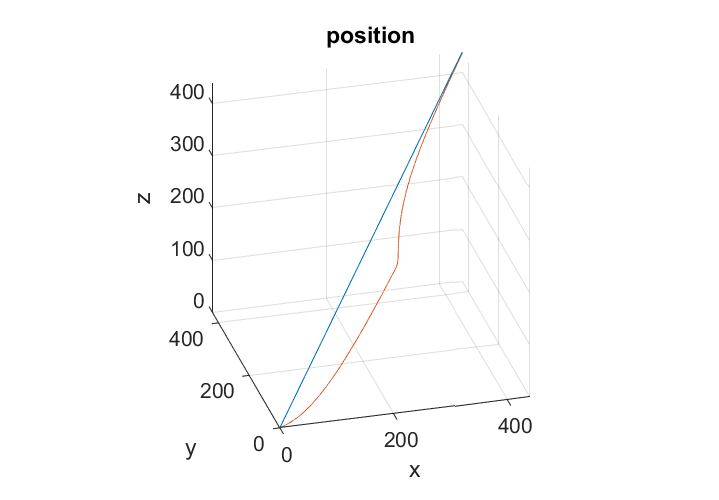
\includegraphics[width = 0.8\linewidth]{Figures/3dlos}
    \caption{LOS guidance in 3D. An offset $\alpha = 40^\circ$ in direction $\theta=160^\circ$ is applied the first half of the simulation, then the offset is turned off and the drone returns to the path.}
    \label{fig:LOS_guidance}
\end{figure}

In addition to the North East Down coordinate system that will generally be used, a $LOS$ coordinate system is defined. This coordinate system is defined as having the x axis along the line between the previous and the next waypoint, denoted as $WP1$ and $WP2$. The y and z axis can be arbitrarily chosen as long as the $LOS$ coordinate system is a right hand coordinate system. The position of $WP_1$ and $WP_2$, and the state of the drone, $x$, are given in the $NED$ frame. The state of the drone consists only of the position and the velocity, $\textbf{x} = \begin{bmatrix} x & y & z & v_x & v_y & v_z\end{bmatrix}^\top$. Note that the line of sight guidance system makes decision based on the current best estimate of the state, $\hat{x}$, not the actual state $x$.

\begin{align}
    x_{LOS} = \frac{WP_2 - WP_1}{||WP_2 - WP_1||} \\
    y_{LOS} = \frac{x_{LOS} \times \begin{bmatrix} 0&0&1\end{bmatrix}^\top}{|| x_{LOS} \times \begin{bmatrix} 0&0&1\end{bmatrix}^\top ||}\label{y_los}\\ 
    z_{LOS} = x_{LOS} \times y_{LOS}
\end{align}

For the special case where $x_{LOS} = \begin{bmatrix} 0&0&1\end{bmatrix}^\top$, where the cross product in \eqref{y_los} is undefined, the alternative formulation is used.

\begin{align}
    x_{LOS} = \frac{WP_2 - WP_1}{||WP_2 - WP_1||} \\
    z_{LOS} = \frac{x_{LOS} \times \begin{bmatrix} 0&1&0\end{bmatrix}^\top}{|| x_{LOS} \times \begin{bmatrix} 0&1&0\end{bmatrix}^\top ||}\\ 
    y_{LOS} = x_{LOS} \times z_{LOS}
\end{align}


\begin{figure*}[t]
\centering
\begin{subfigure}[b]{.48\textwidth}
    \centering
    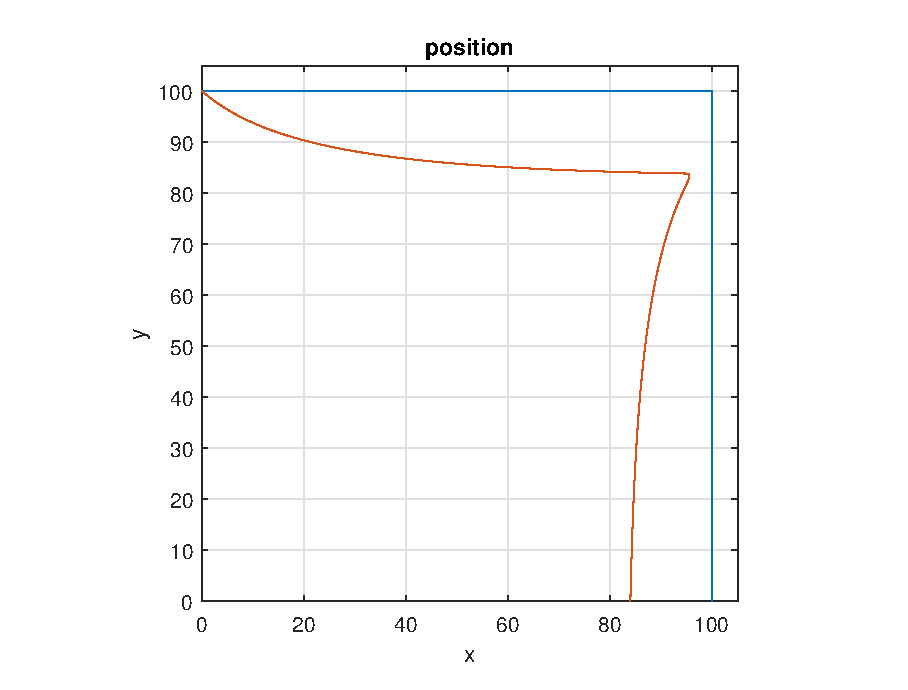
\includegraphics[width = \linewidth]{Figures/gammel_wp_switch}
    \caption{Unwanted behaviour when having switching waypoints based on along path distance. }
    \label{fig:Along_path_switch}
\end{subfigure}
\,
\begin{subfigure}[b]{.48\textwidth}
    \centering
    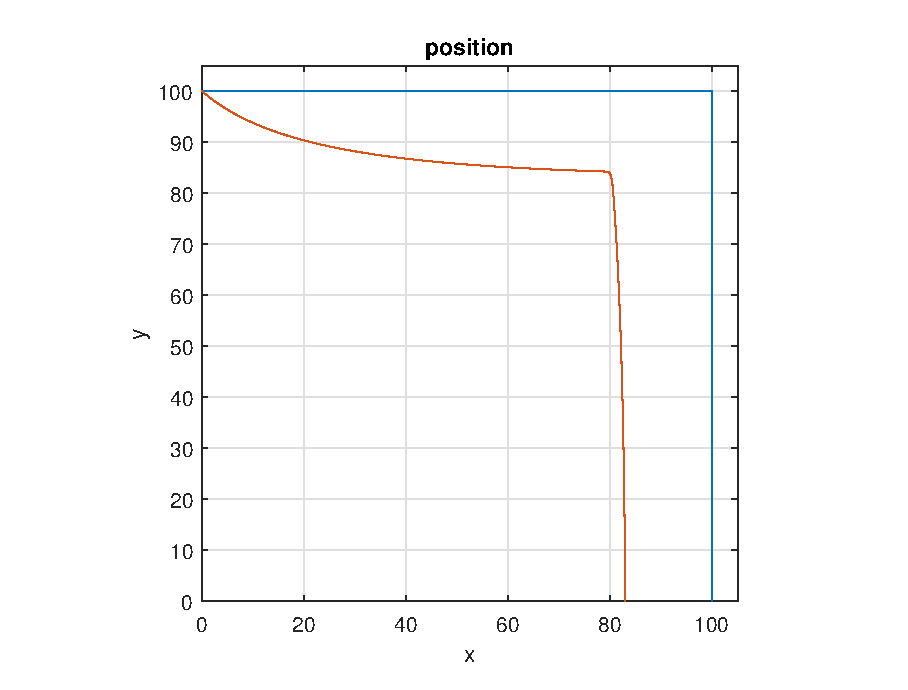
\includegraphics[width = \linewidth]{Figures/ny_wp_switch.eps}
    \caption{Correct behaviour when switching based on relative distance to the two lines.}
    \label{fig:Relative_distance_switch}
\end{subfigure}
\caption{Behaviour with different strategies for changing waypoints. Orange is drone position with a control action offset, blue marks the line between the waypoints.}
\end{figure*}

This basis can be used to find the rotational matrix between $NED$ and $LOS$.
\begin{align}
    R^{NED}_{LOS} = \begin{bmatrix} x_{LOS} & y_{LOS} & z_{LOS}\end{bmatrix}
\end{align}

The difference between $x$ and $WP_1$ given in $LOS$ frame gives the drones offset from the path between the two waypoints. The $x$ coordinate is the distance along the line, while the $y$ and $z$ coordinates gives the offset in $y_{LOS}$ and $z_{LOS}$ direction. The along path distance is irrelevant for LOS guidance so this value will be masked out using an identity matrix with the top left element replaced with a 0. This results in a vector pointing orthogonal out from the path to the drone. LOS guidance makes the drone at all times follow the vector pointing from its current position to a point $\Delta$ ahead on the specified path. In the $LOS$ frame this vector is simply $\Delta$ in $x_{LOS}$ direction and minus the drones distance to $WP_1$ in the $y_{LOS}$ and $z_{LOS}$ direction. By normalizing this vector and multiplying it with the desired speed, $v_0$, the reference speed vector the drone should follow is generated.
\begin{align}
   \chi^{NED}_{LOS} & = R^{NED}_{LOS} \left(  \begin{bmatrix}\Delta \\ 0 \\ 0\end{bmatrix} - \begin{bmatrix} 0 & 0 & 0 \\ 0 & 1 & 0 \\ 0 & 0 & 1 \end{bmatrix} R^{LOS}_{NED} (\begin{bmatrix} \mathbf{I} & \mathbf{0} \end{bmatrix} \hat{\textbf{x}} - WP_1) \right) \label{chi^NED_los} \\
   V_{ref} & = v_0 \frac{\chi^{NED}_{LOS} }{|| \chi^{NED}_{LOS} ||}
\end{align}

The collision avoidance controller wants to add an offset angle the the LOS-vector. In the 2d case an angle $\alpha$ is proposed that is added to the LOS angle. When seen as a vector, this is the same as rotating the vector by $\alpha$ around a z axis pointing out of the paper. For the 3D case two parameters are needed, $\alpha$ and $\theta$. $\alpha$ is used for turning the vector around some axis orthogonal to the $x_{LOS}$ axis. The angle $\theta$ tells us which axis to rotate around. This is done by defining a new coordinate frame with the $x$-axis the same direction as the $LOS$ coordinate frame and the $y$-axis rotated $\theta$ degrees around the $x_{LOS}$-axis. We want to rotate our velocity vector $\alpha$ degrees around the $y$-axis of this new coordinate system. By doing similarity transform we can find the rotational matrix given in $LOS$ frame that results in this rotation. The similarity transform is seen in equation \eqref{R_ca}.



\begin{align}
    \chi^{NED}_{LOS,ca} & =  \label{chi^los_los,ca}\\R^{NED}_{LOS}  R_{ca} &\left(  \begin{bmatrix}\Delta \\ 0 \\ 0\end{bmatrix} - \begin{bmatrix} 0 & 0 & 0 \\ 0 & 1 & 0 \\ 0 & 0 & 1 \end{bmatrix} R^{LOS}_{NED} (\begin{bmatrix} \mathbf{I} & \mathbf{0} \end{bmatrix} \hat{\textbf{x}} - WP_1) \right) \nonumber\\
    R_{ca} & = R_{x=-\theta} R_{y=\alpha} R_{x=\theta} \label{R_ca}\\
    V_{ref,ca} & = v_0 \frac{\chi^{NED}_{LOS,ca} }{|| \chi^{NED}_{LOS,ca} ||} \label{V_ref,ca}
\end{align}


\subsubsection*{Special 2D case}

Since the cross product and rotational matrices around axis are not defined for 2D, the 2D case requires some special notation
\begin{align}
    x_{LOS} = \frac{WP_2 - WP_1}{||WP_2 - WP_1||} \\
    y_{LOS} = \begin{bmatrix}0 & -1\\ 1 & 0 \end{bmatrix} x_{LOS}
\end{align}
\begin{align}
    R^{NED}_{LOS} = \begin{bmatrix} x_{LOS} & y_{LOS} \end{bmatrix}
\end{align}
\begin{align}
    \chi^{NED}_{LOS,ca} & = R^{NED}_{LOS}  R_{ca} \left(  \begin{bmatrix}\Delta \\ 0 \end{bmatrix} - \begin{bmatrix} 0 & 0  \\ 0 & 1  \end{bmatrix} R^{LOS}_{NED} (\begin{bmatrix} \mathbf{I} & \mathbf{0} \end{bmatrix} \hat{\textbf{x}} - WP_1) \right)\\
    R_{ca} & = \begin{bmatrix}cos(\alpha) & -\sin{\alpha}\\ sun(\alpha) & cos(\alpha) \end{bmatrix}
\end{align}

\subsubsection*{Changing between waypoints} \label{wp_change}



Two common way of changing waypoints in line of sight guidance are presented in \cite{Fossen2011}. One mothod is to change waypoint when the vehicle is within a given radius of the waypoint (circle of acceptance). As the control actions might take us far away from the waypoints, this might lead to the waypoint not changing when the vehicle has passed it. The other strategy is to change waypoint when the along path distance to the next waypoint is small enough. This strategy works well when the goal is to follow the desired path closely, but leads to unwanted behaviour when there is an wanted offset due to the control action. The drone might then switch waypoint closer to the next line than the its current offset. The drone will then have to fly further away from the line again to get the correct offset again. This is shown in figure \ref{fig:Along_path_switch}.


The vehicle should instead switch waypoint when it is equally far away from both path-segments. This will avoid making the drone move closer and then further away from the path segment. A margin can be implemented to compensate for the turning dynamic of the drone. The distance to the path segment should be the closest distance to any point of the infinite line going through both waypoints. The distance a point x is along the path $a \rightarrow b$ can be calculated as

\begin{align}
    s(a, b, x) = (x-a)^\top \frac{(b-a)}{||b-a||} \\
\end{align}

The distance left to the next waypoint $WP_n$ is equal the along path distance from the next waypoint to the previous one $WP_{n-1}$. When this distance minus a switch margin, $d$, is smaller than the along path distance from $WP_n$ to $WP_{n+1}$, then the waypoint should be switched, that is $n$ should be increased by one. 

\begin{align}
    s(WP_n, WP_{n-1}) - d \leq s(WP_n WP_{n+1})
\end{align}

The switching margin d should be chosen equal to the stopping distance of the drone. For a $90^\circ$ degree turn, this would require that the drone stops completely in the along path direction, while it builds up speed in the new direction. having a switching margin equal the stop distance would avoid all overshoot. For smaller angles this might lead the the drone switching waypoints a bit early, the smaller the angle is the larger this problem is. But the smaller the angle is the less does it matter if the waypoint is switched earlier, as they close to identical. There will be overshoot if the waypoints have a sharper angle than  $90^\circ$.

The behaviour of this waypoint switching algorithm is shown in figure \ref{fig:Relative_distance_switch}.

\section{Heading dynamic}
For the simplified double integrator drone model, the heading does not affect the position and velocity dynamics, as the drone is able to fly in any direction independent of the heading. But as the sensors are predominantly placed in one direction, the drone is assumed to turn the sensors towards the movement direction to be able to detect obstacles in its way. 

The act of turning collects a lot of data as the sensor cone will gradually move over the obstacles. The moment when the obstacles starts and finishes overlapping the sensor cone will then be registered to give high precision position estimates. A simple heading dynamic is implemented in the simulator to include this behaviour. 

\begin{align}
    \psi &= 0.3 \psi + 0.7 \psi_{ref} \\
    \psi_{ref} &= \textnormal{atan2}(V_{ref,ca,x}, \, V_{ref,ca,y});
\end{align}
